\documentclass{article}
\usepackage[utf8]{inputenc}
\usepackage{fullpage, amsmath, amssymb, amsthm, graphics, graphicx, courier, setspace}
\usepackage{fontenc, hyperref, tikz, float, cancel, subfigure}
\usepackage{fontspec, listings, bm}
\usepackage[shortlabels]{enumitem}


\definecolor{light-gray}{gray}{0.95}
\setmonofont{Courier New}
\lstset{basicstyle=\ttfamily}


\newcommand{\coding}[1]{\colorbox{light-gray}{\texttt{#1}}}
\newcommand{\vect}[2]{$\langle #1, #2 \rangle$}
\newcommand{\pardev}[1]{\frac{\partial}{\partial #1}}
\newcommand{\bb}[3]{\bigg{#1} #3 \bigg{#2}}
\newcommand{\parboth}[2]{\frac{\partial #1}{\partial #2}}

\title{CSC311 Fall 2020\\
	Final Project}
\author{Part A: Jinghao Zhang\\
Part B: Gancheng Luo}
\begin{document}
\maketitle
\newpage

\section*{Part A}
\subsection*{1. k-Nearest Neighbor.}
\subsubsection*{(a) Imputed by student:}
\vspace*{0cm}
\begin{figure*}[htbp]
	\centering
	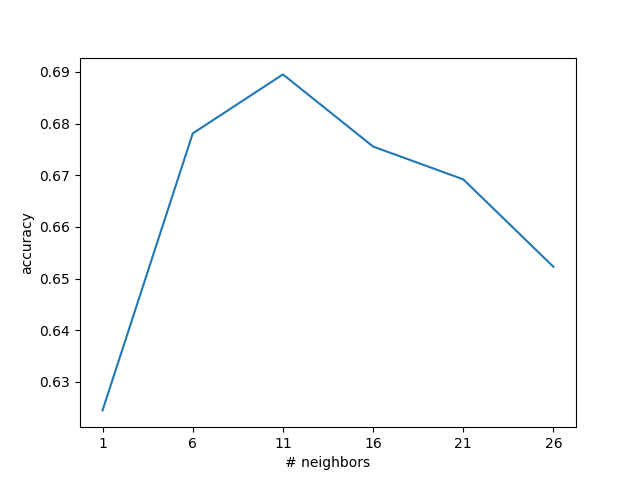
\includegraphics[scale=0.5]{knn_impute_by_student.png}
\end{figure*}
\subsubsection*{(b)}
k = 11 has the best performance, with test accuracy 0.684166
\subsubsection*{(c) Imputed by question:}
\begin{figure*}[htbp]
	\centering
	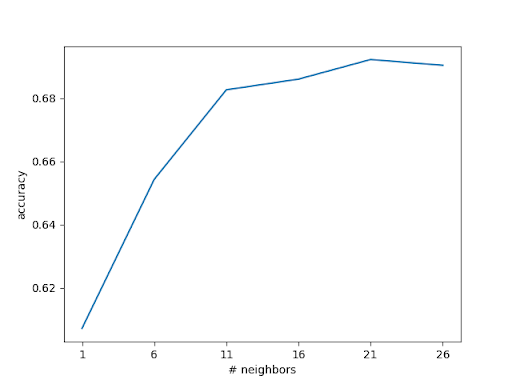
\includegraphics[scale=0.5]{knn_impute_by_question.png}
\end{figure*}
k = 21 has the best performance, with test accuracy 0.681626\\
Assumption for item-based (question-based) collaborative filtering is that if other students have similar correct and incorrect answers on diagnostic questions A and B, then the correctness of specific 
students on questions A and B should match.
\begin{spacing}{1.5} 
\subsubsection*{(d)}
Based on the test performance, user-based collaborative filtering is better, but only by a small margin (68.16 vs 68.42). 
\subsubsection*{(e)}
Notice that both imputations require $k>10$ to reach an optimal level of performance. So, a potential limitation might be sparsity of the data. When knowledge to students performance on the diagnostic
 questions is extremely limited (e.g. when less than 10 neighbors can be found for a data example), the kNN model either runs into error or would not perform as well as expected due to the fact that the
presence of k neighbours is an assumption to kNN.\\ 
Another potential limitation is computational cost. In terms of time complexity, for each of the n total data points of dimension d , kNN takes $\mathcal{O}(nd)$ to calculate the Euclidean distances 
and $\mathcal{O}(n \log n)$ to sort the distances. In addition, since the imputation complements all missing values in a sparse data matrix, considering the fact that multiple values are likely to be missing in a single data example, it might be
 required to take $\mathcal{O}(d (nd + n \log n))$ to replace the missing data entirely. 
\section*{2. Item Response Theory.}
\subsubsection*{(a)}
Denote $$\pi_{i,j} = p(c_{i,j} = 1 | \theta_i, \beta_j) = \frac{\exp(\theta_i - \beta_j)}{1+\exp(\theta_i - \beta_j)}$$ then $p(c_{i,j} | \theta_i, \beta_j) = \pi_{i,j}^{c_{i,j}}\cdot (1-\pi_{i,j})^{1-c_{i,j}}$
log-likelihood: 
\begin{align*}
	l(\theta, \beta) &= \log (p(c| \theta, \beta)) = \log (\prod_i \prod_j p(c_{i,j} | \theta_i, \beta_j))\\
	&= \sum_i \sum_j \log(p(c_{i,j} | \theta_i, \beta_j))\\
	&= \sum_{i,j} \log(\pi_{i,j}^{c_{i,j}}\cdot (1-\pi_{i,j})^{1-c_{i,j}} ) \\
	&= \sum_{i,j} c_{i,j} \log \pi_{i,j} + \sum_{i,j}(1-c_{i,j})\log(1-\pi_{i,j})
\end{align*}
Take derivative \textit{w.r.t} $\theta_j$:
\begin{align*}
	\pardev{\theta_j}l(\theta, \beta) &= \frac{c_{i,j}}{\pi_{i,j}}\cdot\frac{\partial \pi_{i,j}}{\partial \theta_j} - \frac{1-c_{i,j}}{\pi_{i,j}}\cdot\frac{\partial \pi_{i,j}}{\partial \theta_j}\\
	& = \frac{1}{\pi_{i,j}}\cdot\frac{\partial \pi_{i,j}}{\theta_j}\\
	& = \frac{1}{\pi_{i,j}}\cdot \pi_{i,j} \cdot (1-\pi_{i,j})\\
	& = 1- \pi_{i,j} \\ 
	& = \frac{1}{1+\exp(\theta_i- \beta_j)}
\end{align*}
Take derivative \textit{w.r.t} $\beta_j$:
\begin{align*}
	\pardev{\theta_j}l(\theta, \beta) &= \frac{c_{i,j}}{\pi_{i,j}}\cdot\frac{\partial \pi_{i,j}}{\partial \beta_j} - \frac{1-c_{i,j}}{\pi_{i,j}}\cdot\frac{\partial \pi_{i,j}}{\partial \beta_j}\\
	& = \frac{1}{\pi_{i,j}}\cdot \pi_{i,j} \cdot (1-\pi_{i,j})\cdot(-1)\\
	& = \frac{-1}{1+\exp(\theta_i-\beta_j)}
\end{align*}
\subsubsection*{(b)}
Hyperparameters: iterations = 15, learning rate = 0.01
\begin{figure*}[htbp]
	\centering
	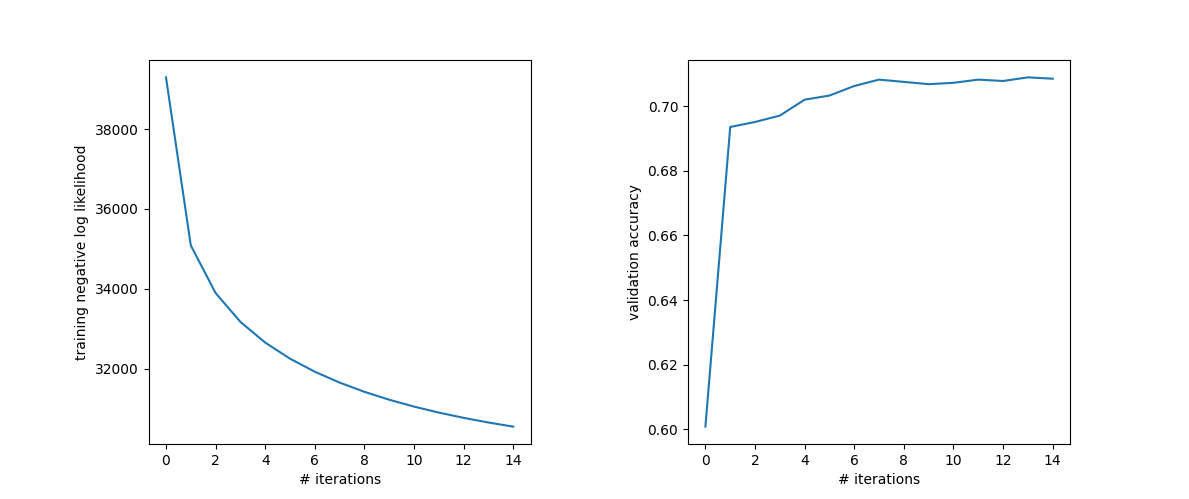
\includegraphics[width=1.1\textwidth]{irt_neg_lld_and_acc.png}
\end{figure*}
\subsubsection*{(c)}
The validation set accuracy is 0.708580. The test accuracy of the trained model is 0.702512.
\subsubsection*{(d)}
\begin{figure*}[htbp]
	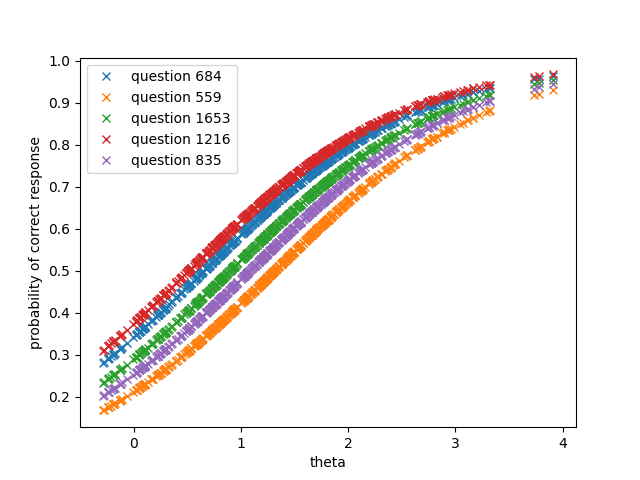
\includegraphics[width=0.8\textwidth]{irt_correctness_probability_with_theta.png}
\end{figure*}
Since we held the question constant, the probability of correct responses increase as the students’ ability $(\theta)$ increases. Observe that there is some degree of resemblance between the graphs and the sigmoid function. 
This is because of the fact that we assumed the probability distribution of correct response given students’ ability and question difficulties has the sigmoid function 
with parameter $(\theta - \beta)$ as its probability density function. Based on this assumption, we trained the model by minimizing the negative log-likelihood (i.e. loss), which is the same as the 
optimization process as in MLE models.
\subsection*{3. Neural Networks.}
\subsubsection*{(a) Difference Between ALS and NN}
ALS solves the problem by decomposing the matrix representation of the data into two matrices of smaller dimensions summarizing the students’ behaviour and the question difficulties, similar to the idea of $\theta$ and $\beta$ 
in item response theory, but in an explicit linear algebra approach. In comparison, a neural network models the problem by attempting to capture the encoding behind the data matrix despite the missing entries, and 
translates/decodes the message into probabilities. \\
ALS provides a way of solving a non-convex objective function (due to the $\bm{u}^\top\bm{z}$ term), whereas objective functions of neural networks are always convex (squared error loss). Also, notice that optimizing the objective 
function for matrix completion is NP-Hard since we want to minimize over two separate vectors. In contrast, the objective function of a neural network only requires optimization over one set of parameters which could 
be computed in linear time using backpropagation.  \\
Due to the fact that it optimizes over two variables, ALS alternates between the two variables when finding the local optimality in the direction of one of the variables, whereas gradients of the loss function in 
neural networks gives the exact direction of the steepest descent with respect to all parameters. However, this does not mean that gradient descent would perform well in the settings of a matrix completion problem. 
On the contrary, gradient descent turns out to converge very slowly when solving such problems. 

\subsubsection*{(d)}
The best set of hyperparameters and optimization hyperparameters are: \coding{$k^*$ = 10, lr = 0.03, num\_epoch = 40}\\
Final validation accuracy = 0.685859, Final test accuracy = 0.688117
\begin{figure*}[htbp]
	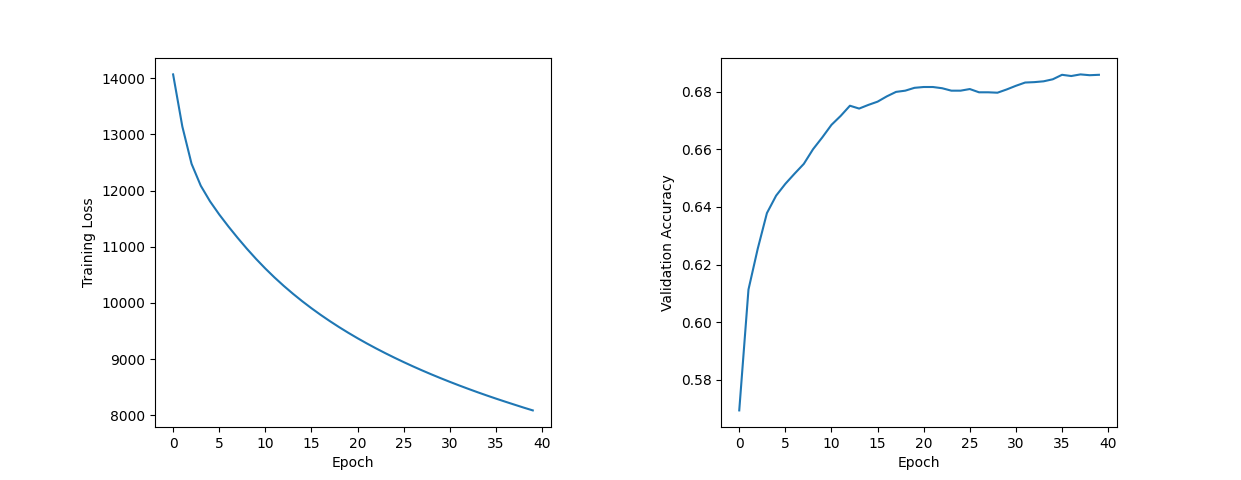
\includegraphics[scale=0.4]{nn_unregularized.png}
\end{figure*}
\subsubsection*{(e)}
The optimal lambda \coding{$\lambda^*$=0.1}
With the same hyperparameter setting, the regularized model performs better in terms of validation accuracy but only by a small margin. The advantage of using regularization penalty is less than 0.005 
validation accuracy. Because of the nature of stochastic gradient descent, the result is not very consistent, and we would conclude that a regularized loss does not significantly improve the performance 
of the autoencoder model. \\
Final validation accuracy = 0.688964\\
Final test accuracy = 0.687835\\
\subsection*{4. Ensemble.}
For ensemble, we used the neural network with regularization penalty from q3 as our base models. The same set of hyperparameters are applied. \\
Ensemble process: first, randomly sample from the training dataset with replacement to obtain the same number of user/student data as the original training set. Repeat the procedure for three times and load 
the sampled data into three separate PyTorch neural network models established in q3. After training with the same hyperparameters, the aggregate prediction is calculated based on majority vote of the predictions 
output by three base models. Then, the averaged prediction is evaluated with respect to the validation data. \\
\\
Final validation accuracy = 0.692210\\
Final test accuracy = 0.686142\\\\
Over multiple runs of the ensemble model, a consistent improvement from the base models can be observed in terms of validation accuracy. But the increase in performance is still minimal, at approximately 
0.005 validation accuracy. However, the predictions output by ensemble are more stable and have less variance in comparison to the neural network base model. Due to the fact that ensemble compensated for the 
impact of SGD (by reducing variance), we would conclude that ensemble has a better performance over previous models. 
\newpage
\section*{Part B}
\subsection*{1. Description.}
We decide to extend the Neural Network model by adding 2 layers. Now given a user $\bm{v}\in \mathbb{R}^{N_{\text{questions}}}$ from the user set $\mathcal{S}$, we want to: 
\[\min_{\bm{\theta}} \sum_{\bm{v} \in \mathcal{S}}||\bm{v} - f(\bm{v}; \bm{\theta})||_2^2 + \frac{\lambda}{2}\bb{(}{)}{||\bm{W}^{(1)}||_F^2 + ||\bm{W}^{(2)}||_F^2 + ||\bm{W}^{(3)}||_F^2 +||\bm{W}^{(4)}||_F^2}\], where 
\[f(\bm{v}; \bm{\theta}) =l(\bm{W}^{(4)}k(\bm{W}^{(3)}h(\bm{W}^{(2)}g(\bm{W}^{(1)}\bm{v}+\bm{b}^{(1)})+\bm{b}^{(2)})+\bm{b}^{(3)})+\bm{b}^{(4)}) \]
We want to increase the number of layers because with only one layer the model might not be able to capture enough detail from the data, which means the model is underfitting. With more layers, the model will be more 
expressive and able to learn more details. As a result, we will see an higher validation accuracy. 
\subsection*{2. Figure or Diagram.}
The diagram of the model is as follows: 
\begin{figure*}[htbp]
	\centering
	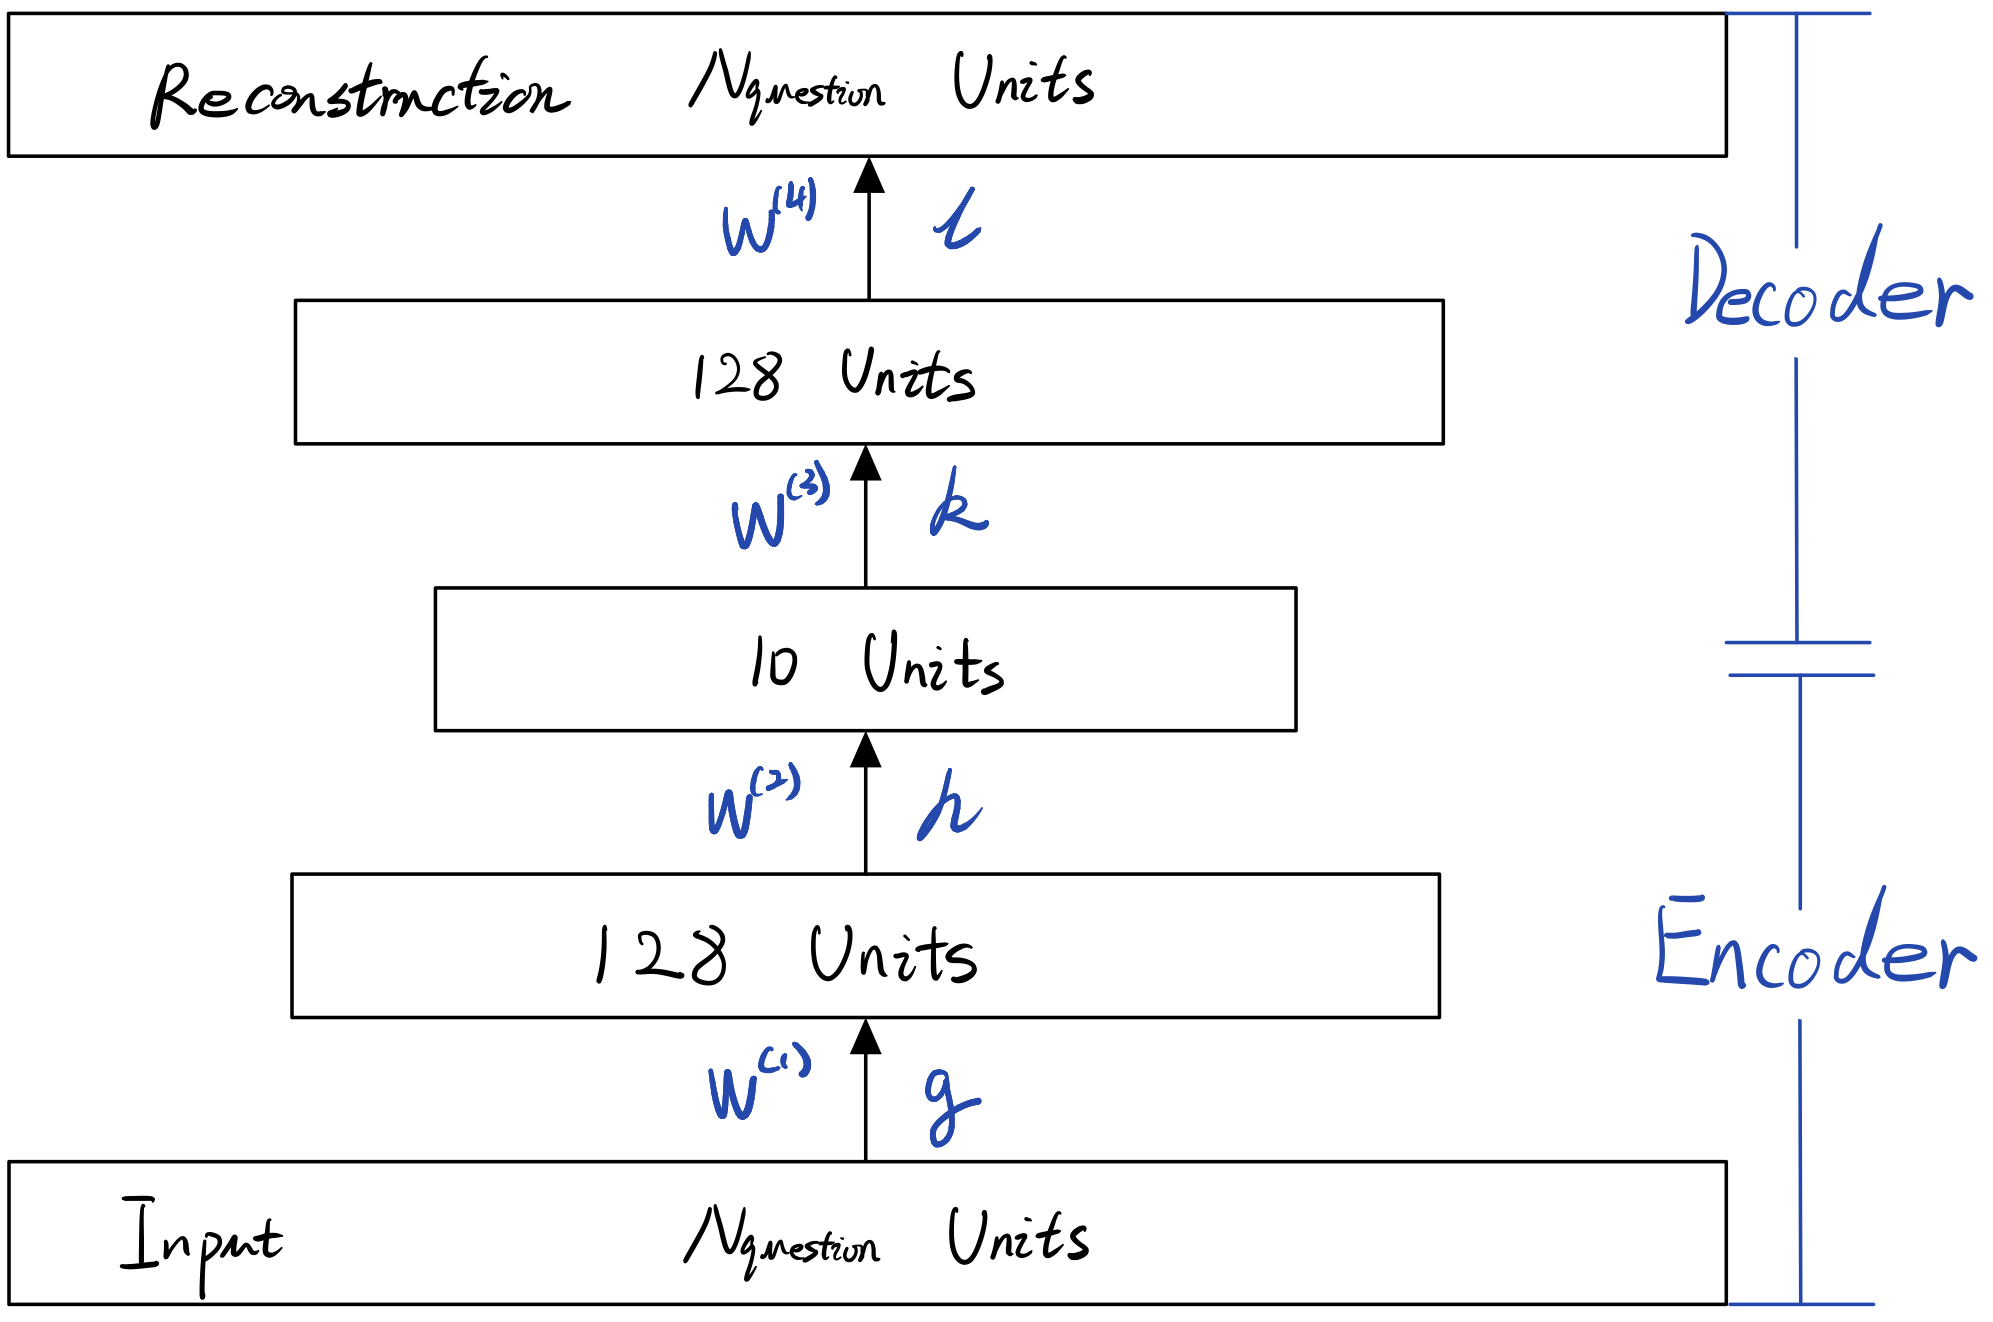
\includegraphics[width=0.7\textwidth]{nnModel.png}
\end{figure*}\\
As for the other hyperparameters, we use the settings that \coding{$\lambda$=0.01, lr = 0.03, epoch=45} and \coding{sigmoid} activation.
\subsection*{3. Comparison or Demonstration.}
On the left is accuracy plot for the basic model, on the right is the extended one.
\begin{figure}[H]
    \begin{minipage}[b]{0.5\linewidth}
        \centering
		\includegraphics[width=1\textwidth]{nn/base.png}
		\caption{Basic Model}
    \end{minipage}
    \begin{minipage}[b]{0.5\linewidth}
        \centering
		\includegraphics[width=1\textwidth]{nn/128-10.png}
		\caption{\# units in first layer: 128, second layer: 10}
    \end{minipage}
\end{figure}
As for the test accuracy, the basic one is \coding{68.5577\%} while the extended one is \coding{70.1101\%}. We see such improvement because more layers help the model learn more imformation from the data. \\
To find the best combination of number of units in the layers, we tried some combinations and finally decide to use \coding{128, 10}.
\begin{figure}[H]
    \begin{minipage}[b]{0.5\linewidth}
        \centering
		\includegraphics[width=1\textwidth]{starter_code/part_a/64-16.png}
		\caption{\# units in first layer: 64, second layer: 16}
    \end{minipage}
    \begin{minipage}[b]{0.5\linewidth}
        \centering
		\includegraphics[width=1\textwidth]{starter_code/part_a/512-10.png}
		\caption{\# units in first layer: 512, second layer: 10}
    \end{minipage}
\end{figure}
\subsection*{4. Limitations.}
In a setting where students and question have more than one attribute to differentiate one from another instead of just id, ALS and NN will be very likely to perform poorly. A major drawback of ALS and autoencoder NN 
is that we can hardly incorprate other information of students and questions with the 2D matrix in addition to their ids.\\
If we want to consider the effect of age, gender or the fields they good at on the ability to answer different fields of questions, it is hard to make such a matrix that can let ALS or NN work well with. 
And AlS and autoencoder are established based on the dimensionality of the 2D matrix. Even if we can somehow aplly the algorithm to some "3D" matrix, the complexity of the model will increase dramatically. 
The space and time cost of the computation will also see an explanation increase.\\
A possible solution is that we can somehow wrap all information and maybe lower the dimension to make the computation feasible.




\end{spacing}
\end{document}